\subsection{Příklad}

Následující příklad je převzat ze \textit{Sbírky příkladů stavební mechaniky} \cite[Příklad 5.2]{sbirka_prikladu}.

\begin{figure}[H]
    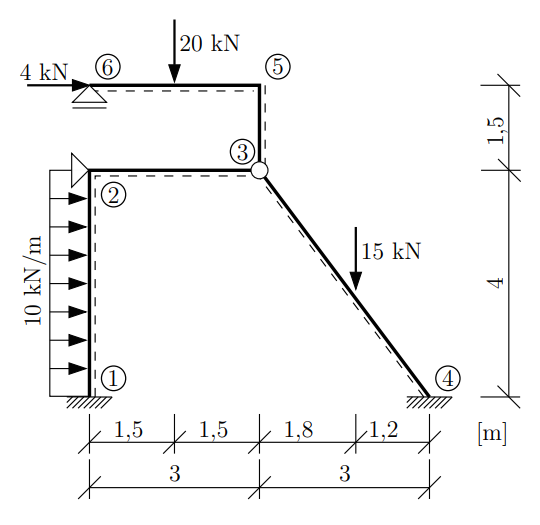
\includegraphics[height=7cm]{assets/figures/framesss/example_snk.png}
    \caption[Statické schéma konstrukce]{Statické schéma konstrukce, převzato z \cite[Příklad 5.2]{sbirka_prikladu}}
    \label{fig:framesss_example}
\end{figure}

Všechny pruty mají Youngův modul pružnosti $\gls{E} = \SI{30}{\GPa}$, moment setrvačnosti k ose, kolem které jsou pruty namáhané ohybem $\gls{I_y} = \SI{1e-3}{\unit{\metre\tothe{4}}}$ a plochu $\gls{A}= \SI{4e-3}{{\metre\tothe{2}}}$.

Na příkladu bude ilustrováno použití knihovny \texttt{framesss} v prostředí JupyterLab.

V prvním kroku je nutné importovat knihovny, se kterými budeme pracovat.

\begin{tcolorbox}[breakable, size=fbox, boxrule=1pt, pad at break*=1mm,colback=cellbackground, colframe=cellborder]
    \prompt{In}{incolor}{1}{\boxspacing}
    \begin{Verbatim}[commandchars=\\\{\}]
    \PY{k+kn}{import} \PY{n+nn}{numpy} \PY{k}{as} \PY{n+nn}{np}
    
    \PY{k+kn}{from} \PY{n+nn}{tabulate} \PY{k+kn}{import} \PY{n}{tabulate}
    
    \PY{k+kn}{from} \PY{n+nn}{framesss}\PY{n+nn}{.}\PY{n+nn}{fea}\PY{n+nn}{.}\PY{n+nn}{models}\PY{n+nn}{.}\PY{n+nn}{frame\PYZus{}xz} \PY{k+kn}{import} \PY{n}{FrameXZModel}
    \PY{k+kn}{from} \PY{n+nn}{framesss}\PY{n+nn}{.}\PY{n+nn}{pre}\PY{n+nn}{.}\PY{n+nn}{material} \PY{k+kn}{import} \PY{n}{Material}
    \PY{k+kn}{from} \PY{n+nn}{framesss}\PY{n+nn}{.}\PY{n+nn}{pre}\PY{n+nn}{.}\PY{n+nn}{section} \PY{k+kn}{import} \PY{n}{Section}
    \PY{k+kn}{from} \PY{n+nn}{framesss}\PY{n+nn}{.}\PY{n+nn}{solvers}\PY{n+nn}{.}\PY{n+nn}{linear\PYZus{}static} \PY{k+kn}{import} \PY{n}{LinearStaticSolver}
    \end{Verbatim}
\end{tcolorbox}

Začneme definicí materiálu, knihovna nepracuje s převody jednotek, musíme být konzistentní. Zvolíme systém jednotek $\text{kN, kPa a m}$. Poissonův součinitel \gls{nu}, teplotní součinitel roztažnosti, ani objemovou hmotnost materiálu bychom nemuseli definovat, protože mají výchozí hodnoty, ale uvádíme je zde pro přehlednost.
\begin{tcolorbox}[breakable, size=fbox, boxrule=1pt, pad at break*=1mm,colback=cellbackground, colframe=cellborder]
    \prompt{In}{incolor}{2}{\boxspacing}
    \begin{Verbatim}[commandchars=\\\{\}]
    \PY{n}{material} \PY{o}{=} \PY{n}{Material}\PY{p}{(}
        \PY{n}{label}\PY{o}{=}\PY{l+s+s2}{\PYZdq{}}\PY{l+s+s2}{foo}\PY{l+s+s2}{\PYZdq{}}\PY{p}{,}
        \PY{n}{elastic\PYZus{}modulus}\PY{o}{=}\PY{l+m+mf}{30.e6}\PY{p}{,}
        \PY{n}{poissons\PYZus{}ratio}\PY{o}{=}\PY{l+m+mf}{0.2}\PY{p}{,}
        \PY{n}{thermal\PYZus{}expansion\PYZus{}coefficient}\PY{o}{=}\PY{l+m+mf}{1.0e\PYZhy{}3}\PY{p}{,}
        \PY{n}{density}\PY{o}{=}\PY{l+m+mf}{0.0}\PY{p}{,}
    \PY{p}{)}
    \end{Verbatim}
\end{tcolorbox}

Jako další definujeme průřez prvku pomocí třídy \texttt{Section}, proměnná \texttt{area\_x} slouží pro výpočet normálové tuhosti, \texttt{area\_y} a \texttt{area\_z} se ve výpočtu použijí pouze v případě, že prutový prvek, kterému tento průřez přiřadíme bude typu \texttt{'timoshenko'}. Plocha zadaná těmto atributům má odpovídat hodnotě $k \gls{A}$, kde k je korekční součinitel rozložení smykového napětí. Pro získání správného výsledku je dále potřeba přiřadit správnou hodnotu momentu setrvačnosti \gls{I_y} do atributu \texttt{inertia\_y} a přiřadit materiál definovaný v předchozí buňce, ostatní hodnoty při tomto výpočtu nehrají roli, uvádíme je pouze pro přehlednost.
\begin{tcolorbox}[breakable, size=fbox, boxrule=1pt, pad at break*=1mm,colback=cellbackground, colframe=cellborder]
    \prompt{In}{incolor}{3}{\boxspacing}
    \begin{Verbatim}[commandchars=\\\{\}]
    \PY{n}{section} \PY{o}{=} \PY{n}{Section}\PY{p}{(}
        \PY{n}{label}\PY{o}{=}\PY{l+s+s2}{\PYZdq{}}\PY{l+s+s2}{bar}\PY{l+s+s2}{\PYZdq{}}\PY{p}{,}
        \PY{n}{area\PYZus{}x}\PY{o}{=}\PY{l+m+mf}{4.0e\PYZhy{}3}\PY{p}{,}
        \PY{n}{area\PYZus{}y}\PY{o}{=}\PY{l+m+mf}{1.0}\PY{p}{,}
        \PY{n}{area\PYZus{}z}\PY{o}{=}\PY{l+m+mf}{1.0}\PY{p}{,}
        \PY{n}{inertia\PYZus{}x}\PY{o}{=}\PY{l+m+mf}{1.0}\PY{p}{,}
        \PY{n}{inertia\PYZus{}y}\PY{o}{=}\PY{l+m+mf}{1.0e\PYZhy{}3}\PY{p}{,}
        \PY{n}{inertia\PYZus{}z}\PY{o}{=}\PY{l+m+mf}{1.0}\PY{p}{,}
        \PY{n}{height\PYZus{}z}\PY{o}{=}\PY{l+m+mf}{1.0}\PY{p}{,}
        \PY{n}{height\PYZus{}y}\PY{o}{=}\PY{l+m+mf}{1.0}\PY{p}{,}
        \PY{n}{material}\PY{o}{=}\PY{n}{material}
    \PY{p}{)}
    \end{Verbatim}
\end{tcolorbox}

V dalším kroku vytvoříme instanci modelu \texttt{FrameXZModel}. Pomocí metod této třídy budeme modelovat celou konstrukci i se zatížením.
\begin{tcolorbox}[breakable, size=fbox, boxrule=1pt, pad at break*=1mm,colback=cellbackground, colframe=cellborder]
    \prompt{In}{incolor}{4}{\boxspacing}
    \begin{Verbatim}[commandchars=\\\{\}]
    \PY{n}{model} \PY{o}{=} \PY{n}{FrameXZModel}\PY{p}{(}\PY{p}{)}
    \end{Verbatim}
\end{tcolorbox}

Pomocí metody \texttt{add\_node()} definujeme uzly konstrukce. Atributy, které musíme zadat jsou označení uzlu \texttt{label} a souřadnice uzlu \texttt{coords} ve formátu [\gls{X}, \gls{Y}, \gls{Z}]. Nepovinným atributem metody je \texttt{fixity}, kterou definujeme okrajové podmínky pro každý stupeň volnosti v uzlu, zadáváme je pomocí stringů \texttt{'fixed'} nebo \texttt{'free'} a řadíme je v pořadí [\gls{u_i}[ ], \gls{v_i}[ ], \gls{w_i}[ ], \gls{phi_i}[\gls{x}], \gls{phi_i}[\gls{y}], \gls{phi_i}[\gls{z}]].
\begin{tcolorbox}[breakable, size=fbox, boxrule=1pt, pad at break*=1mm,colback=cellbackground, colframe=cellborder]
    \prompt{In}{incolor}{5}{\boxspacing}
    \begin{Verbatim}[commandchars=\\\{\}]
    \PY{n}{N1} \PY{o}{=} \PY{n}{model}\PY{o}{.}\PY{n}{add\PYZus{}node}\PY{p}{(}
        \PY{n}{label}\PY{o}{=}\PY{l+s+s2}{\PYZdq{}}\PY{l+s+s2}{N1}\PY{l+s+s2}{\PYZdq{}}\PY{p}{,}
        \PY{n}{coords}\PY{o}{=}\PY{p}{[}\PY{l+m+mf}{0.0}\PY{p}{,} \PY{l+m+mf}{0.0}\PY{p}{,} \PY{l+m+mf}{0.0}\PY{p}{]}\PY{p}{,}
        \PY{n}{fixity}\PY{o}{=}\PY{p}{[}\PY{l+s+s1}{\PYZsq{}}\PY{l+s+s1}{fixed}\PY{l+s+s1}{\PYZsq{}}\PY{p}{,} \PY{l+s+s1}{\PYZsq{}}\PY{l+s+s1}{free}\PY{l+s+s1}{\PYZsq{}}\PY{p}{,} \PY{l+s+s1}{\PYZsq{}}\PY{l+s+s1}{fixed}\PY{l+s+s1}{\PYZsq{}}\PY{p}{,} \PY{l+s+s1}{\PYZsq{}}\PY{l+s+s1}{free}\PY{l+s+s1}{\PYZsq{}}\PY{p}{,} \PY{l+s+s1}{\PYZsq{}}\PY{l+s+s1}{fixed}\PY{l+s+s1}{\PYZsq{}}\PY{p}{,} \PY{l+s+s1}{\PYZsq{}}\PY{l+s+s1}{free}\PY{l+s+s1}{\PYZsq{}}\PY{p}{]}\PY{p}{,}
    \PY{p}{)}
    
    \PY{n}{N2} \PY{o}{=} \PY{n}{model}\PY{o}{.}\PY{n}{add\PYZus{}node}\PY{p}{(}
        \PY{n}{label}\PY{o}{=}\PY{l+s+s2}{\PYZdq{}}\PY{l+s+s2}{N2}\PY{l+s+s2}{\PYZdq{}}\PY{p}{,}
        \PY{n}{coords}\PY{o}{=}\PY{p}{[}\PY{l+m+mf}{0.0}\PY{p}{,} \PY{l+m+mf}{0.0}\PY{p}{,} \PY{l+m+mf}{4.0}\PY{p}{]}\PY{p}{,}
        \PY{n}{fixity}\PY{o}{=}\PY{p}{[}\PY{l+s+s2}{\PYZdq{}}\PY{l+s+s2}{fixed}\PY{l+s+s2}{\PYZdq{}}\PY{p}{,} \PY{l+s+s2}{\PYZdq{}}\PY{l+s+s2}{free}\PY{l+s+s2}{\PYZdq{}}\PY{p}{,} \PY{l+s+s2}{\PYZdq{}}\PY{l+s+s2}{fixed}\PY{l+s+s2}{\PYZdq{}}\PY{p}{,} \PY{l+s+s2}{\PYZdq{}}\PY{l+s+s2}{free}\PY{l+s+s2}{\PYZdq{}}\PY{p}{,} \PY{l+s+s2}{\PYZdq{}}\PY{l+s+s2}{free}\PY{l+s+s2}{\PYZdq{}}\PY{p}{,} \PY{l+s+s2}{\PYZdq{}}\PY{l+s+s2}{free}\PY{l+s+s2}{\PYZdq{}}\PY{p}{]}\PY{p}{,}
    \PY{p}{)}
    
    \PY{n}{N3} \PY{o}{=} \PY{n}{model}\PY{o}{.}\PY{n}{add\PYZus{}node}\PY{p}{(}
        \PY{n}{label}\PY{o}{=}\PY{l+s+s2}{\PYZdq{}}\PY{l+s+s2}{N3}\PY{l+s+s2}{\PYZdq{}}\PY{p}{,}
        \PY{n}{coords}\PY{o}{=}\PY{p}{[}\PY{l+m+mf}{3.0}\PY{p}{,} \PY{l+m+mf}{0.0}\PY{p}{,} \PY{l+m+mf}{4.0}\PY{p}{]}\PY{p}{,}
    \PY{p}{)}
    
    \PY{n}{N4} \PY{o}{=} \PY{n}{model}\PY{o}{.}\PY{n}{add\PYZus{}node}\PY{p}{(}
        \PY{n}{label}\PY{o}{=}\PY{l+s+s2}{\PYZdq{}}\PY{l+s+s2}{N4}\PY{l+s+s2}{\PYZdq{}}\PY{p}{,}
        \PY{n}{coords}\PY{o}{=}\PY{p}{[}\PY{l+m+mf}{6.0}\PY{p}{,} \PY{l+m+mf}{0.0}\PY{p}{,} \PY{l+m+mf}{0.0}\PY{p}{]}\PY{p}{,}
        \PY{n}{fixity}\PY{o}{=}\PY{p}{[}\PY{l+s+s2}{\PYZdq{}}\PY{l+s+s2}{fixed}\PY{l+s+s2}{\PYZdq{}}\PY{p}{,} \PY{l+s+s2}{\PYZdq{}}\PY{l+s+s2}{free}\PY{l+s+s2}{\PYZdq{}}\PY{p}{,} \PY{l+s+s2}{\PYZdq{}}\PY{l+s+s2}{fixed}\PY{l+s+s2}{\PYZdq{}}\PY{p}{,} \PY{l+s+s2}{\PYZdq{}}\PY{l+s+s2}{free}\PY{l+s+s2}{\PYZdq{}}\PY{p}{,} \PY{l+s+s2}{\PYZdq{}}\PY{l+s+s2}{fixed}\PY{l+s+s2}{\PYZdq{}}\PY{p}{,} \PY{l+s+s2}{\PYZdq{}}\PY{l+s+s2}{free}\PY{l+s+s2}{\PYZdq{}}\PY{p}{]}
    \PY{p}{)}
    
    \PY{n}{N5} \PY{o}{=} \PY{n}{model}\PY{o}{.}\PY{n}{add\PYZus{}node}\PY{p}{(}
        \PY{n}{label}\PY{o}{=}\PY{l+s+s2}{\PYZdq{}}\PY{l+s+s2}{N5}\PY{l+s+s2}{\PYZdq{}}\PY{p}{,}
        \PY{n}{coords}\PY{o}{=}\PY{p}{[}\PY{l+m+mf}{3.0}\PY{p}{,} \PY{l+m+mf}{0.0}\PY{p}{,} \PY{l+m+mf}{5.5}\PY{p}{]}\PY{p}{,}
    \PY{p}{)}
    
    \PY{n}{N6} \PY{o}{=} \PY{n}{model}\PY{o}{.}\PY{n}{add\PYZus{}node}\PY{p}{(}
        \PY{n}{label}\PY{o}{=}\PY{l+s+s2}{\PYZdq{}}\PY{l+s+s2}{N6}\PY{l+s+s2}{\PYZdq{}}\PY{p}{,}
        \PY{n}{coords}\PY{o}{=}\PY{p}{[}\PY{l+m+mf}{0.0}\PY{p}{,} \PY{l+m+mf}{0.0}\PY{p}{,} \PY{l+m+mf}{5.5}\PY{p}{]}\PY{p}{,}
        \PY{n}{fixity}\PY{o}{=}\PY{p}{[}\PY{l+s+s1}{\PYZsq{}}\PY{l+s+s1}{free}\PY{l+s+s1}{\PYZsq{}}\PY{p}{,} \PY{l+s+s1}{\PYZsq{}}\PY{l+s+s1}{free}\PY{l+s+s1}{\PYZsq{}}\PY{p}{,} \PY{l+s+s1}{\PYZsq{}}\PY{l+s+s1}{fixed}\PY{l+s+s1}{\PYZsq{}}\PY{p}{,} \PY{l+s+s1}{\PYZsq{}}\PY{l+s+s1}{free}\PY{l+s+s1}{\PYZsq{}}\PY{p}{,} \PY{l+s+s1}{\PYZsq{}}\PY{l+s+s1}{free}\PY{l+s+s1}{\PYZsq{}}\PY{p}{,} \PY{l+s+s1}{\PYZsq{}}\PY{l+s+s1}{free}\PY{l+s+s1}{\PYZsq{}}\PY{p}{]}
    \PY{p}{)}
    \end{Verbatim}
\end{tcolorbox}

Pomocí metody \texttt{add\_member()} přidáme jednotlivé pruty. Atributy jsou označení \texttt{label}, typ použitého elementu \texttt{element\_type}, který může být buď \texttt{'navier'} pro prut bez vlivu smyku nebo \texttt{'timoshenko'} pro prut s vlivem smyku. Dále zadáme počáteční a koncový uzel, průřez prvku a můžeme zadat nepovinný atribut \texttt{hinges}, který udává, zda je v odpovídajícím uzlu prut připojen kloubově nebo pevně.
\begin{tcolorbox}[breakable, size=fbox, boxrule=1pt, pad at break*=1mm,colback=cellbackground, colframe=cellborder]
    \prompt{In}{incolor}{6}{\boxspacing}
    \begin{Verbatim}[commandchars=\\\{\}]
    \PY{n}{B12} \PY{o}{=} \PY{n}{model}\PY{o}{.}\PY{n}{add\PYZus{}member}\PY{p}{(}
        \PY{n}{label}\PY{o}{=}\PY{l+s+s2}{\PYZdq{}}\PY{l+s+s2}{1\PYZhy{}2}\PY{l+s+s2}{\PYZdq{}}\PY{p}{,}
        \PY{n}{element\PYZus{}type}\PY{o}{=}\PY{l+s+s2}{\PYZdq{}}\PY{l+s+s2}{navier}\PY{l+s+s2}{\PYZdq{}}\PY{p}{,}
        \PY{n}{nodes}\PY{o}{=}\PY{p}{[}\PY{n}{N1}\PY{p}{,} \PY{n}{N2}\PY{p}{]}\PY{p}{,}
        \PY{n}{section}\PY{o}{=}\PY{n}{section}\PY{p}{,}
    \PY{p}{)}
    
    \PY{n}{B23} \PY{o}{=} \PY{n}{model}\PY{o}{.}\PY{n}{add\PYZus{}member}\PY{p}{(}
        \PY{n}{label}\PY{o}{=}\PY{l+s+s2}{\PYZdq{}}\PY{l+s+s2}{2\PYZhy{}3}\PY{l+s+s2}{\PYZdq{}}\PY{p}{,}
        \PY{n}{element\PYZus{}type}\PY{o}{=}\PY{l+s+s2}{\PYZdq{}}\PY{l+s+s2}{navier}\PY{l+s+s2}{\PYZdq{}}\PY{p}{,}
        \PY{n}{nodes}\PY{o}{=}\PY{p}{[}\PY{n}{N2}\PY{p}{,} \PY{n}{N3}\PY{p}{]}\PY{p}{,}
        \PY{n}{section}\PY{o}{=}\PY{n}{section}\PY{p}{,}
        \PY{n}{hinges}\PY{o}{=}\PY{p}{[}\PY{l+s+s2}{\PYZdq{}}\PY{l+s+s2}{fixed}\PY{l+s+s2}{\PYZdq{}}\PY{p}{,} \PY{l+s+s2}{\PYZdq{}}\PY{l+s+s2}{hinged}\PY{l+s+s2}{\PYZdq{}}\PY{p}{]}\PY{p}{,}
    \PY{p}{)}
    
    \PY{n}{B34} \PY{o}{=} \PY{n}{model}\PY{o}{.}\PY{n}{add\PYZus{}member}\PY{p}{(}
        \PY{n}{label}\PY{o}{=}\PY{l+s+s2}{\PYZdq{}}\PY{l+s+s2}{3\PYZhy{}4}\PY{l+s+s2}{\PYZdq{}}\PY{p}{,}
        \PY{n}{element\PYZus{}type}\PY{o}{=}\PY{l+s+s2}{\PYZdq{}}\PY{l+s+s2}{navier}\PY{l+s+s2}{\PYZdq{}}\PY{p}{,}
        \PY{n}{nodes}\PY{o}{=}\PY{p}{[}\PY{n}{N3}\PY{p}{,} \PY{n}{N4}\PY{p}{]}\PY{p}{,}
        \PY{n}{section}\PY{o}{=}\PY{n}{section}\PY{p}{,}
        \PY{n}{hinges}\PY{o}{=}\PY{p}{[}\PY{l+s+s2}{\PYZdq{}}\PY{l+s+s2}{hinged}\PY{l+s+s2}{\PYZdq{}}\PY{p}{,} \PY{l+s+s2}{\PYZdq{}}\PY{l+s+s2}{fixed}\PY{l+s+s2}{\PYZdq{}}\PY{p}{]}\PY{p}{,}
    \PY{p}{)}
    
    \PY{n}{B35} \PY{o}{=} \PY{n}{model}\PY{o}{.}\PY{n}{add\PYZus{}member}\PY{p}{(}
        \PY{n}{label}\PY{o}{=}\PY{l+s+s2}{\PYZdq{}}\PY{l+s+s2}{3\PYZhy{}5}\PY{l+s+s2}{\PYZdq{}}\PY{p}{,}
        \PY{n}{element\PYZus{}type}\PY{o}{=}\PY{l+s+s2}{\PYZdq{}}\PY{l+s+s2}{navier}\PY{l+s+s2}{\PYZdq{}}\PY{p}{,}
        \PY{n}{nodes}\PY{o}{=}\PY{p}{[}\PY{n}{N3}\PY{p}{,} \PY{n}{N5}\PY{p}{]}\PY{p}{,}
        \PY{n}{section}\PY{o}{=}\PY{n}{section}\PY{p}{,}
        \PY{n}{hinges}\PY{o}{=}\PY{p}{[}\PY{l+s+s2}{\PYZdq{}}\PY{l+s+s2}{hinged}\PY{l+s+s2}{\PYZdq{}}\PY{p}{,} \PY{l+s+s2}{\PYZdq{}}\PY{l+s+s2}{fixed}\PY{l+s+s2}{\PYZdq{}}\PY{p}{]}\PY{p}{,}
    \PY{p}{)}
    
    \PY{n}{B65} \PY{o}{=} \PY{n}{model}\PY{o}{.}\PY{n}{add\PYZus{}member}\PY{p}{(}
        \PY{n}{label}\PY{o}{=}\PY{l+s+s2}{\PYZdq{}}\PY{l+s+s2}{6\PYZhy{}5}\PY{l+s+s2}{\PYZdq{}}\PY{p}{,}
        \PY{n}{element\PYZus{}type}\PY{o}{=}\PY{l+s+s2}{\PYZdq{}}\PY{l+s+s2}{navier}\PY{l+s+s2}{\PYZdq{}}\PY{p}{,}
        \PY{n}{nodes}\PY{o}{=}\PY{p}{[}\PY{n}{N6}\PY{p}{,} \PY{n}{N5}\PY{p}{]}\PY{p}{,}
        \PY{n}{section}\PY{o}{=}\PY{n}{section}\PY{p}{,}
    \PY{p}{)}
    \end{Verbatim}
\end{tcolorbox}

V dalším kroku definujeme zatížení. Zatěžovací stav do modelu přidáme pomocí metody \texttt{add\_load\_case()}. Jednotlivé síly a spojitá zatížení přidáváme přímo na dříve definované instance prutů a uzlů pomocí metod \texttt{add\_distributed\_load()} a \texttt{add\_point\_load()} pro pruty, případně \texttt{add\_nodal\_load()} pro uzly. Výchozí směr zatížení je v globálním souřadném systému. Polohu spojitého zatížení zadáváme pomocí atributů \texttt{x\_start} a \texttt{x\_end}, hodnoty zadáváme hodnotou na začátku a na konci intervalu pro směry \gls{x}, \gls{y} a \gls{z}. Tímto přístupem je možné modelovat lichoběžníkové zatížení kdekoliv na nosníku. Pomocí metody \texttt{add\_point\_load()} lze přidat osamělou sílu nebo moment, hodnoty musí být v pořadí $[F_{\gls{x}}, F_{\gls{y}}, F_{\gls{z}}, M_{\gls{x}}, M_{\gls{y}}, M_{\gls{z}}]$.
\begin{tcolorbox}[breakable, size=fbox, boxrule=1pt, pad at break*=1mm,colback=cellbackground, colframe=cellborder]
    \prompt{In}{incolor}{7}{\boxspacing}
    \begin{Verbatim}[commandchars=\\\{\}]
        \PY{n}{LC1} \PY{o}{=} \PY{n}{model}\PY{o}{.}\PY{n}{add\PYZus{}load\PYZus{}case}\PY{p}{(}
            \PY{n}{label}\PY{o}{=}\PY{l+s+s1}{\PYZsq{}}\PY{l+s+s1}{LC1}\PY{l+s+s1}{\PYZsq{}}
        \PY{p}{)}
        
        \PY{n}{B12}\PY{o}{.}\PY{n}{add\PYZus{}distributed\PYZus{}load}\PY{p}{(}
            \PY{n}{load\PYZus{}components}\PY{o}{=}\PY{p}{[}\PY{l+m+mf}{10.}\PY{p}{,} \PY{l+m+mf}{0.}\PY{p}{,} \PY{l+m+mf}{0.}\PY{p}{,} \PY{l+m+mf}{10.}\PY{p}{,} \PY{l+m+mf}{0.}\PY{p}{,} \PY{l+m+mf}{0.}\PY{p}{]}\PY{p}{,}
            \PY{n}{load\PYZus{}case}\PY{o}{=}\PY{n}{LC1}\PY{p}{,}
            \PY{n}{x\PYZus{}start}\PY{o}{=}\PY{l+m+mf}{0.0}\PY{p}{,}
            \PY{n}{x\PYZus{}end}\PY{o}{=}\PY{l+m+mf}{1.0}\PY{p}{,}
            \PY{n}{coordinate\PYZus{}system}\PY{o}{=}\PY{l+s+s2}{\PYZdq{}}\PY{l+s+s2}{global}\PY{l+s+s2}{\PYZdq{}}\PY{p}{,}
            \PY{n}{location}\PY{o}{=}\PY{l+s+s2}{\PYZdq{}}\PY{l+s+s2}{length}\PY{l+s+s2}{\PYZdq{}}\PY{p}{,}
            \PY{n}{coordinate\PYZus{}definition}\PY{o}{=}\PY{l+s+s2}{\PYZdq{}}\PY{l+s+s2}{relative}\PY{l+s+s2}{\PYZdq{}}\PY{p}{,}
        \PY{p}{)}
        
        \PY{n}{B34}\PY{o}{.}\PY{n}{add\PYZus{}point\PYZus{}load}\PY{p}{(}
            \PY{n}{load\PYZus{}components}\PY{o}{=}\PY{p}{[}\PY{l+m+mf}{0.}\PY{p}{,} \PY{l+m+mf}{0.}\PY{p}{,} \PY{o}{\PYZhy{}}\PY{l+m+mf}{15.}\PY{p}{,} \PY{l+m+mf}{0.}\PY{p}{,} \PY{l+m+mf}{0.}\PY{p}{,} \PY{l+m+mf}{0.}\PY{p}{]}\PY{p}{,}
            \PY{n}{load\PYZus{}case}\PY{o}{=}\PY{n}{LC1}\PY{p}{,}
            \PY{n}{x}\PY{o}{=}\PY{l+m+mf}{1.8}\PY{o}{/}\PY{l+m+mi}{3}\PY{p}{,}
            \PY{n}{coordinate\PYZus{}system}\PY{o}{=}\PY{l+s+s2}{\PYZdq{}}\PY{l+s+s2}{global}\PY{l+s+s2}{\PYZdq{}}\PY{p}{,}
            \PY{n}{coordinate\PYZus{}definition}\PY{o}{=}\PY{l+s+s2}{\PYZdq{}}\PY{l+s+s2}{relative}\PY{l+s+s2}{\PYZdq{}}\PY{p}{,}
        \PY{p}{)}
        
        \PY{n}{B65}\PY{o}{.}\PY{n}{add\PYZus{}point\PYZus{}load}\PY{p}{(}
            \PY{n}{load\PYZus{}components}\PY{o}{=}\PY{p}{[}\PY{l+m+mf}{0.}\PY{p}{,} \PY{l+m+mf}{0.}\PY{p}{,} \PY{o}{\PYZhy{}}\PY{l+m+mf}{20.}\PY{p}{,} \PY{l+m+mf}{0.}\PY{p}{,} \PY{l+m+mf}{0.}\PY{p}{,} \PY{l+m+mf}{0.}\PY{p}{]}\PY{p}{,}
            \PY{n}{load\PYZus{}case}\PY{o}{=}\PY{n}{LC1}\PY{p}{,}
            \PY{n}{x}\PY{o}{=}\PY{l+m+mf}{0.5}\PY{p}{,}
        \PY{p}{)}
        
        \PY{n}{N6}\PY{o}{.}\PY{n}{add\PYZus{}nodal\PYZus{}load}\PY{p}{(}
            \PY{n}{load\PYZus{}components}\PY{o}{=}\PY{p}{[}\PY{l+m+mf}{4.}\PY{p}{,} \PY{l+m+mf}{0.}\PY{p}{,} \PY{l+m+mf}{0.}\PY{p}{,} \PY{l+m+mf}{0.}\PY{p}{,} \PY{l+m+mf}{0.}\PY{p}{,} \PY{l+m+mf}{0.}\PY{p}{]}\PY{p}{,}
            \PY{n}{load\PYZus{}case}\PY{o}{=}\PY{n}{LC1}\PY{p}{,}
        \PY{p}{)}
    \end{Verbatim}
\end{tcolorbox}

To samé zatížení přidáme do modelu ještě jednou, tentokrát však každé zatížení přiřadíme jinému zatěžovacímu stavu, poté z jednotlivých stavů vytvoříme novou kombinaci zatížení. Hodnoty zatížení vydělíme součiniteli \texttt{LC<i>\_factor} a při vytváření nové kombinace tento součinitel použijeme jako součinitel kombinace.
\begin{tcolorbox}[breakable, size=fbox, boxrule=1pt, pad at break*=1mm,colback=cellbackground, colframe=cellborder]
    \prompt{In}{incolor}{8}{\boxspacing}
    \begin{Verbatim}[commandchars=\\\{\}]
    \PY{n}{LC2\PYZus{}factor} \PY{o}{=} \PY{l+m+mi}{2}
    \PY{n}{LC3\PYZus{}factor} \PY{o}{=} \PY{l+m+mi}{18}
    \PY{n}{LC4\PYZus{}factor} \PY{o}{=} \PY{l+m+mf}{5.5}
    \PY{n}{LC5\PYZus{}factor} \PY{o}{=} \PY{o}{\PYZhy{}}\PY{l+m+mi}{12}
    
    \PY{n}{LC2} \PY{o}{=} \PY{n}{model}\PY{o}{.}\PY{n}{add\PYZus{}load\PYZus{}case}\PY{p}{(}
        \PY{n}{label}\PY{o}{=}\PY{l+s+s2}{\PYZdq{}}\PY{l+s+s2}{LC2}\PY{l+s+s2}{\PYZdq{}}
    \PY{p}{)}
    \PY{n}{B12}\PY{o}{.}\PY{n}{add\PYZus{}distributed\PYZus{}load}\PY{p}{(}
        \PY{n}{load\PYZus{}components}\PY{o}{=}\PY{n}{np}\PY{o}{.}\PY{n}{array}\PY{p}{(}
            \PY{p}{[}\PY{l+m+mf}{10.}\PY{p}{,} \PY{l+m+mf}{0.}\PY{p}{,} \PY{l+m+mf}{0.}\PY{p}{,} \PY{l+m+mf}{10.}\PY{p}{,} \PY{l+m+mf}{0.}\PY{p}{,} \PY{l+m+mf}{0.}\PY{p}{]}
        \PY{p}{)} \PY{o}{/} \PY{n}{LC2\PYZus{}factor}\PY{p}{,}
        \PY{n}{load\PYZus{}case}\PY{o}{=}\PY{n}{LC2}\PY{p}{,}
    \PY{p}{)}
    
    \PY{n}{LC3} \PY{o}{=} \PY{n}{model}\PY{o}{.}\PY{n}{add\PYZus{}load\PYZus{}case}\PY{p}{(}
        \PY{n}{label}\PY{o}{=}\PY{l+s+s2}{\PYZdq{}}\PY{l+s+s2}{LC3}\PY{l+s+s2}{\PYZdq{}}
    \PY{p}{)}
    \PY{n}{B34}\PY{o}{.}\PY{n}{add\PYZus{}point\PYZus{}load}\PY{p}{(}
        \PY{n}{load\PYZus{}components}\PY{o}{=}\PY{n}{np}\PY{o}{.}\PY{n}{array}\PY{p}{(}
            \PY{p}{[}\PY{l+m+mf}{0.}\PY{p}{,} \PY{l+m+mf}{0.}\PY{p}{,} \PY{o}{\PYZhy{}}\PY{l+m+mf}{15.}\PY{p}{,} \PY{l+m+mf}{0.}\PY{p}{,} \PY{l+m+mf}{0.}\PY{p}{,} \PY{l+m+mf}{0.}\PY{p}{]}
        \PY{p}{)} \PY{o}{/} \PY{n}{LC3\PYZus{}factor}\PY{p}{,}
        \PY{n}{load\PYZus{}case}\PY{o}{=}\PY{n}{LC3}\PY{p}{,}
        \PY{n}{x}\PY{o}{=}\PY{l+m+mf}{1.8}\PY{o}{/}\PY{l+m+mi}{3}\PY{p}{,}
    \PY{p}{)}
    
    \PY{n}{LC4} \PY{o}{=}  \PY{n}{model}\PY{o}{.}\PY{n}{add\PYZus{}load\PYZus{}case}\PY{p}{(}
        \PY{n}{label}\PY{o}{=}\PY{l+s+s2}{\PYZdq{}}\PY{l+s+s2}{LC4}\PY{l+s+s2}{\PYZdq{}}
    \PY{p}{)}
    \PY{n}{B65}\PY{o}{.}\PY{n}{add\PYZus{}point\PYZus{}load}\PY{p}{(}
        \PY{n}{load\PYZus{}components}\PY{o}{=}\PY{n}{np}\PY{o}{.}\PY{n}{array}\PY{p}{(}
            \PY{p}{[}\PY{l+m+mf}{0.}\PY{p}{,} \PY{l+m+mf}{0.}\PY{p}{,} \PY{o}{\PYZhy{}}\PY{l+m+mf}{20.}\PY{p}{,} \PY{l+m+mf}{0.}\PY{p}{,} \PY{l+m+mf}{0.}\PY{p}{,} \PY{l+m+mf}{0.}\PY{p}{]}
        \PY{p}{)} \PY{o}{/} \PY{n}{LC4\PYZus{}factor}\PY{p}{,}
        \PY{n}{load\PYZus{}case}\PY{o}{=}\PY{n}{LC4}\PY{p}{,}
        \PY{n}{x}\PY{o}{=}\PY{l+m+mf}{0.5}\PY{p}{,}
    \PY{p}{)}
    
    \PY{n}{LC5} \PY{o}{=} \PY{n}{model}\PY{o}{.}\PY{n}{add\PYZus{}load\PYZus{}case}\PY{p}{(}
        \PY{n}{label}\PY{o}{=}\PY{l+s+s2}{\PYZdq{}}\PY{l+s+s2}{LC5}\PY{l+s+s2}{\PYZdq{}}
    \PY{p}{)}
    \PY{n}{N6}\PY{o}{.}\PY{n}{add\PYZus{}nodal\PYZus{}load}\PY{p}{(}
        \PY{n}{load\PYZus{}components}\PY{o}{=}\PY{n}{np}\PY{o}{.}\PY{n}{array}\PY{p}{(}
            \PY{p}{[}\PY{l+m+mf}{4.}\PY{p}{,} \PY{l+m+mf}{0.}\PY{p}{,} \PY{l+m+mf}{0.}\PY{p}{,} \PY{l+m+mf}{0.}\PY{p}{,} \PY{l+m+mf}{0.}\PY{p}{,} \PY{l+m+mf}{0.}\PY{p}{]}
        \PY{p}{)} \PY{o}{/} \PY{n}{LC5\PYZus{}factor}\PY{p}{,}
        \PY{n}{load\PYZus{}case}\PY{o}{=}\PY{n}{LC5}\PY{p}{,}
    \PY{p}{)}
    
    \PY{n}{CO1} \PY{o}{=} \PY{n}{model}\PY{o}{.}\PY{n}{add\PYZus{}load\PYZus{}case\PYZus{}combination}\PY{p}{(}
        \PY{n}{label}\PY{o}{=}\PY{l+s+s2}{\PYZdq{}}\PY{l+s+s2}{CO1}\PY{l+s+s2}{\PYZdq{}}\PY{p}{,}
        \PY{n}{combination}\PY{o}{=}\PY{p}{\PYZob{}}
            \PY{n}{LC2}\PY{p}{:} \PY{n}{LC2\PYZus{}factor}\PY{p}{,}
            \PY{n}{LC3}\PY{p}{:} \PY{n}{LC3\PYZus{}factor}\PY{p}{,}
            \PY{n}{LC4}\PY{p}{:} \PY{n}{LC4\PYZus{}factor}\PY{p}{,}
            \PY{n}{LC5}\PY{p}{:} \PY{n}{LC5\PYZus{}factor}\PY{p}{,}
        \PY{p}{\PYZcb{}}
    \PY{p}{)}
    \end{Verbatim}
\end{tcolorbox}

Vytvoříme instanci řešiče a propojíme ho s instancí \texttt{model}.
\begin{tcolorbox}[breakable, size=fbox, boxrule=1pt, pad at break*=1mm,colback=cellbackground, colframe=cellborder]
    \prompt{In}{incolor}{9}{\boxspacing}
    \begin{Verbatim}[commandchars=\\\{\}]
    \PY{n}{solver} \PY{o}{=} \PY{n}{LinearStaticSolver}\PY{p}{(}
        \PY{n}{model}\PY{o}{=}\PY{n}{model}
    \PY{p}{)}
    \end{Verbatim}
\end{tcolorbox}

Výpočet provedeme pomocí metody \texttt{solve()}.
\begin{tcolorbox}[breakable, size=fbox, boxrule=1pt, pad at break*=1mm,colback=cellbackground, colframe=cellborder]
    \prompt{In}{incolor}{10}{\boxspacing}
    \begin{Verbatim}[commandchars=\\\{\}]
    \PY{n}{solver}\PY{o}{.}\PY{n}{solve}\PY{p}{(}\PY{p}{)}
    \end{Verbatim}
\end{tcolorbox}

Výsledky jsou uložené v instancích tříd \texttt{Node} a \texttt{Member1D} v objektu \texttt{results}. Pomocí metody {get()}, dostaneme výsledky pro zatěžovací stavy nebo kombinace. Hodnoty nakonec vypíšeme do tabulky. V tabulce si můžeme všimnout, že program vytvořil vlastní uzly v místech působících osamělých sil.
\begin{tcolorbox}[breakable, size=fbox, boxrule=1pt, pad at break*=1mm,colback=cellbackground, colframe=cellborder]
    \prompt{In}{incolor}{11}{\boxspacing}
    \begin{Verbatim}[commandchars=\\\{\}]
    \PY{n}{displacements}\PY{o}{=} \PY{p}{[}\PY{p}{]}
    \PY{n}{reactions} \PY{o}{=} \PY{p}{[}\PY{p}{]}
    \PY{k}{for} \PY{n}{node} \PY{o+ow}{in} \PY{n}{model}\PY{o}{.}\PY{n}{nodes}\PY{p}{:}
        \PY{k}{for} \PY{n}{case} \PY{o+ow}{in} \PY{p}{[}\PY{n}{LC1}\PY{p}{,} \PY{n}{CO1}\PY{p}{]}\PY{p}{:}
            \PY{n}{displacements}\PY{o}{.}\PY{n}{append}\PY{p}{(}\PY{p}{[}
                \PY{k}{case}\PY{o}{.}\PY{n}{label}\PY{p}{,}
                \PY{n}{node}\PY{o}{.}\PY{n}{label}\PY{p}{,}
                \PY{n}{node}\PY{o}{.}\PY{n}{results}\PY{o}{.}\PY{n}{translation\PYZus{}x}\PY{o}{.}\PY{n}{get}\PY{p}{(}\PY{n}{case}\PY{p}{)}\PY{p}{,}
                \PY{n}{node}\PY{o}{.}\PY{n}{results}\PY{o}{.}\PY{n}{translation\PYZus{}z}\PY{o}{.}\PY{n}{get}\PY{p}{(}\PY{n}{case}\PY{p}{)}\PY{p}{,}
                \PY{n}{node}\PY{o}{.}\PY{n}{results}\PY{o}{.}\PY{n}{rotation\PYZus{}y}\PY{o}{.}\PY{n}{get}\PY{p}{(}\PY{n}{case}\PY{p}{)}\PY{p}{,}
            \PY{p}{]}\PY{p}{)}
            \PY{n}{r\PYZus{}x} \PY{o}{=} \PY{n}{node}\PY{o}{.}\PY{n}{results}\PY{o}{.}\PY{n}{reaction\PYZus{}force\PYZus{}x}\PY{o}{.}\PY{n}{get}\PY{p}{(}\PY{n}{case}\PY{p}{)}
            \PY{n}{r\PYZus{}z} \PY{o}{=} \PY{n}{node}\PY{o}{.}\PY{n}{results}\PY{o}{.}\PY{n}{reaction\PYZus{}force\PYZus{}z}\PY{o}{.}\PY{n}{get}\PY{p}{(}\PY{n}{case}\PY{p}{)}
            \PY{n}{r\PYZus{}my} \PY{o}{=} \PY{n}{node}\PY{o}{.}\PY{n}{results}\PY{o}{.}\PY{n}{reaction\PYZus{}moment\PYZus{}y}\PY{o}{.}\PY{n}{get}\PY{p}{(}\PY{n}{case}\PY{p}{)}
    
            \PY{k}{if} \PY{n}{r\PYZus{}x} \PY{o+ow}{or} \PY{n}{r\PYZus{}z} \PY{o+ow}{or} \PY{n}{r\PYZus{}my}\PY{p}{:}
                \PY{n}{reactions}\PY{o}{.}\PY{n}{append}\PY{p}{(}\PY{p}{[}
                    \PY{k}{case}\PY{o}{.}\PY{n}{label}\PY{p}{,}
                    \PY{n}{node}\PY{o}{.}\PY{n}{label}\PY{p}{,}
                    \PY{n}{r\PYZus{}x}\PY{p}{,}
                    \PY{n}{r\PYZus{}z}\PY{p}{,}
                    \PY{n}{r\PYZus{}my}
                \PY{p}{]}\PY{p}{)}
            
        \PY{n}{displacements}\PY{o}{.}\PY{n}{append}\PY{p}{(}\PY{p}{[}\PY{k+kc}{None}\PY{p}{]} \PY{o}{*} \PY{l+m+mi}{5}\PY{p}{)}
        \PY{k}{if} \PY{n}{r\PYZus{}x} \PY{o+ow}{or} \PY{n}{r\PYZus{}z} \PY{o+ow}{or} \PY{n}{r\PYZus{}my}\PY{p}{:}
            \PY{n}{reactions}\PY{o}{.}\PY{n}{append}\PY{p}{(}\PY{p}{[}\PY{k+kc}{None}\PY{p}{]} \PY{o}{*} \PY{l+m+mi}{5}\PY{p}{)}
    
    \PY{n+nb}{print}\PY{p}{(}\PY{n}{tabulate}\PY{p}{(}
        \PY{n}{displacements}\PY{p}{,}
        \PY{n}{headers}\PY{o}{=}\PY{p}{[}\PY{l+s+s2}{\PYZdq{}}\PY{l+s+s2}{case}\PY{l+s+s2}{\PYZdq{}}\PY{p}{,} \PY{l+s+s2}{\PYZdq{}}\PY{l+s+s2}{node}\PY{l+s+s2}{\PYZdq{}}\PY{p}{,} \PY{l+s+s2}{\PYZdq{}}\PY{l+s+s2}{u\PYZus{}x}\PY{l+s+s2}{\PYZdq{}}\PY{p}{,} \PY{l+s+s2}{\PYZdq{}}\PY{l+s+s2}{u\PYZus{}z}\PY{l+s+s2}{\PYZdq{}}\PY{p}{,} \PY{l+s+s2}{\PYZdq{}}\PY{l+s+s2}{phi\PYZus{}y}\PY{l+s+s2}{\PYZdq{}}\PY{p}{]}\PY{p}{,}
        \PY{n}{tablefmt}\PY{o}{=}\PY{l+s+s2}{\PYZdq{}}\PY{l+s+s2}{rst}\PY{l+s+s2}{\PYZdq{}}\PY{p}{,}
        \PY{n}{floatfmt}\PY{o}{=}\PY{l+s+s2}{\PYZdq{}}\PY{l+s+s2}{.3e}\PY{l+s+s2}{\PYZdq{}}
    \PY{p}{)}\PY{p}{)}
    \PY{n+nb}{print}\PY{p}{(}\PY{n}{tabulate}\PY{p}{(}
        \PY{n}{reactions}\PY{p}{,}
        \PY{n}{headers}\PY{o}{=}\PY{p}{[}\PY{l+s+s2}{\PYZdq{}}\PY{l+s+s2}{case}\PY{l+s+s2}{\PYZdq{}}\PY{p}{,} \PY{l+s+s2}{\PYZdq{}}\PY{l+s+s2}{node}\PY{l+s+s2}{\PYZdq{}}\PY{p}{,} \PY{l+s+s2}{\PYZdq{}}\PY{l+s+s2}{R\PYZus{}x}\PY{l+s+s2}{\PYZdq{}}\PY{p}{,} \PY{l+s+s2}{\PYZdq{}}\PY{l+s+s2}{R\PYZus{}z}\PY{l+s+s2}{\PYZdq{}}\PY{p}{,} \PY{l+s+s2}{\PYZdq{}}\PY{l+s+s2}{R\PYZus{}My}\PY{l+s+s2}{\PYZdq{}}\PY{p}{]}\PY{p}{,}
        \PY{n}{tablefmt}\PY{o}{=}\PY{l+s+s2}{\PYZdq{}}\PY{l+s+s2}{rst}\PY{l+s+s2}{\PYZdq{}}\PY{p}{,}
        \PY{n}{floatfmt}\PY{o}{=}\PY{l+s+s2}{\PYZdq{}}\PY{l+s+s2}{.3f}\PY{l+s+s2}{\PYZdq{}}
    \PY{p}{)}\PY{p}{)}
    \end{Verbatim}
    \end{tcolorbox}
    
\begin{Verbatim}[commandchars=\\\{\}]
    ======  ======  ==========  ==========  ==========
    case    node           u\_x         u\_z       phi\_y
    ======  ======  ==========  ==========  ==========
    LC1     N1       0.000e+00   0.000e+00   0.000e+00
    CO1     N1       0.000e+00   0.000e+00   0.000e+00

    LC1     N2       0.000e+00   0.000e+00  -6.942e-05
    CO1     N2       0.000e+00   0.000e+00  -6.942e-05
    
    LC1     N3      -9.902e-05  -9.168e-04   0.000e+00
    CO1     N3      -9.902e-05  -9.168e-04   0.000e+00

    LC1     N4       0.000e+00   0.000e+00   0.000e+00
    CO1     N4       0.000e+00   0.000e+00   0.000e+00
    
    LC1     N5       3.219e-04  -1.067e-03   1.806e-04
    CO1     N5       3.219e-04  -1.067e-03   1.806e-04
    
    LC1     N6       4.219e-04   0.000e+00   6.306e-04
    CO1     N6       4.219e-04   0.000e+00   6.306e-04
        
    LC1     3-4(1)  -7.831e-05  -5.457e-04  -2.216e-04
    CO1     3-4(1)  -7.831e-05  -5.457e-04  -2.216e-04
    
    LC1     6-5(1)   3.719e-04  -7.959e-04   3.306e-04
    CO1     6-5(1)   3.719e-04  -7.959e-04   3.306e-04

    ======  ======  ==========  ==========  ==========

    ======  ======  =======  ======  =======
    case    node        R\_x     R\_z     R\_My
    ======  ======  =======  ======  =======
    LC1     N1      -20.781   0.000  -14.375
    CO1     N1      -20.781   0.000  -14.375
     
    LC1     N2      -15.258   3.750
    CO1     N2      -15.258   3.750

    LC1     N4       -7.961  23.250   10.905
    CO1     N4       -7.961  23.250   10.905

    LC1     N6                8.000
    CO1     N6                8.000
    ======  ======  =======  ======  =======
        \end{Verbatim}
    

\begin{figure}[H]
    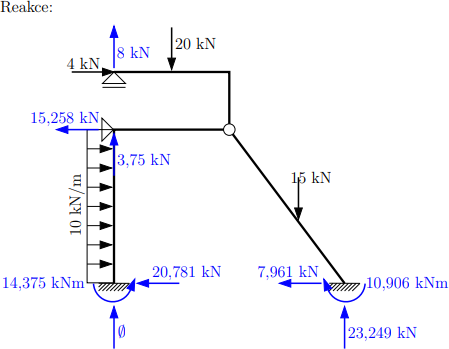
\includegraphics{assets/figures/framesss/example_reactions.png}
    \caption[Reakce v podporách]{Reakce v podporách, převzato z \cite[Příklad 5.2]{sbirka_prikladu}}
    \label{fig:framesss_example_reactions}
\end{figure}

    Stejně jako v případu uzlů, výsledky se ukládají do objektu \texttt{results}, do tabulky vypíšeme extrémy vnitřních sil pro jednotlivé prvky.
        \begin{tcolorbox}[breakable, size=fbox, boxrule=1pt, pad at break*=1mm,colback=cellbackground, colframe=cellborder]
    \prompt{In}{incolor}{12}{\boxspacing}
    \begin{Verbatim}[commandchars=\\\{\}]
    \PY{n}{headers} \PY{o}{=} \PY{p}{[}\PY{l+s+s2}{\PYZdq{}}\PY{l+s+s2}{case}\PY{l+s+s2}{\PYZdq{}}\PY{p}{,} \PY{l+s+s2}{\PYZdq{}}\PY{l+s+s2}{member}\PY{l+s+s2}{\PYZdq{}}\PY{p}{,} \PY{l+s+s2}{\PYZdq{}}\PY{l+s+s2}{N\PYZus{}min}\PY{l+s+s2}{\PYZdq{}}\PY{p}{,} \PY{l+s+s2}{\PYZdq{}}\PY{l+s+s2}{N\PYZus{}max}\PY{l+s+s2}{\PYZdq{}}\PY{p}{,} \PY{l+s+s2}{\PYZdq{}}\PY{l+s+s2}{V\PYZus{}min}\PY{l+s+s2}{\PYZdq{}}\PY{p}{,} \PY{l+s+s1}{\PYZsq{}}\PY{l+s+s1}{V\PYZus{}max}\PY{l+s+s1}{\PYZsq{}}\PY{p}{,} \PY{l+s+s2}{\PYZdq{}}\PY{l+s+s2}{M\PYZus{}min}\PY{l+s+s2}{\PYZdq{}}\PY{p}{,} \PY{l+s+s2}{\PYZdq{}}\PY{l+s+s2}{M\PYZus{}max}\PY{l+s+s2}{\PYZdq{}}\PY{p}{]}
    \PY{n}{axial} \PY{o}{=} \PY{p}{[}\PY{p}{]}
    \PY{n}{shear} \PY{o}{=} \PY{p}{[}\PY{p}{]}
    \PY{n}{moment} \PY{o}{=} \PY{p}{[}\PY{p}{]}
    \PY{k}{for} \PY{n}{member} \PY{o+ow}{in} \PY{n}{model}\PY{o}{.}\PY{n}{members}\PY{p}{:}
        \PY{k}{for} \PY{n}{case} \PY{o+ow}{in} \PY{p}{[}\PY{n}{LC1}\PY{p}{,} \PY{n}{CO1}\PY{p}{]}\PY{p}{:}
            \PY{n}{axial}\PY{o}{.}\PY{n}{append}\PY{p}{(}\PY{p}{[}
                \PY{k}{case}\PY{o}{.}\PY{n}{label}\PY{p}{,}
                \PY{n}{member}\PY{o}{.}\PY{n}{label}\PY{p}{,}
                \PY{o}{*}\PY{n}{member}\PY{o}{.}\PY{n}{results}\PY{o}{.}\PY{n}{min\PYZus{}max\PYZus{}axial\PYZus{}forces}\PY{o}{.}\PY{n}{get}\PY{p}{(}\PY{n}{case}\PY{p}{)}\PY{o}{.}\PY{n}{tolist}\PY{p}{(}\PY{p}{)}
            \PY{p}{]}\PY{p}{)}
            \PY{n}{shear}\PY{o}{.}\PY{n}{append}\PY{p}{(}\PY{p}{[}
                \PY{k}{case}\PY{o}{.}\PY{n}{label}\PY{p}{,}
                \PY{n}{member}\PY{o}{.}\PY{n}{label}\PY{p}{,}
                \PY{o}{*}\PY{n}{member}\PY{o}{.}\PY{n}{results}\PY{o}{.}\PY{n}{min\PYZus{}max\PYZus{}shear\PYZus{}forces\PYZus{}z}\PY{o}{.}\PY{n}{get}\PY{p}{(}\PY{n}{case}\PY{p}{)}\PY{o}{.}\PY{n}{tolist}\PY{p}{(}\PY{p}{)}
            \PY{p}{]}\PY{p}{)}
            \PY{n}{moment}\PY{o}{.}\PY{n}{append}\PY{p}{(}\PY{p}{[}
                \PY{k}{case}\PY{o}{.}\PY{n}{label}\PY{p}{,}
                \PY{n}{member}\PY{o}{.}\PY{n}{label}\PY{p}{,}
                \PY{o}{*}\PY{n}{member}\PY{o}{.}\PY{n}{results}\PY{o}{.}\PY{n}{min\PYZus{}max\PYZus{}bending\PYZus{}moments\PYZus{}y}\PY{o}{.}\PY{n}{get}\PY{p}{(}\PY{n}{case}\PY{p}{)}\PY{o}{.}\PY{n}{tolist}\PY{p}{(}\PY{p}{)}
            \PY{p}{]}\PY{p}{)}
        \PY{n}{axial}\PY{o}{.}\PY{n}{append}\PY{p}{(}\PY{p}{[}\PY{k+kc}{None}\PY{p}{]} \PY{o}{*} \PY{l+m+mi}{2}\PY{p}{)}
        \PY{n}{shear}\PY{o}{.}\PY{n}{append}\PY{p}{(}\PY{p}{[}\PY{k+kc}{None}\PY{p}{]} \PY{o}{*} \PY{l+m+mi}{2}\PY{p}{)}
        \PY{n}{moment}\PY{o}{.}\PY{n}{append}\PY{p}{(}\PY{p}{[}\PY{k+kc}{None}\PY{p}{]} \PY{o}{*} \PY{l+m+mi}{2}\PY{p}{)}
    
    \PY{k}{for} \PY{n}{i}\PY{p}{,} \PY{n}{data} \PY{o+ow}{in} \PY{n+nb}{enumerate}\PY{p}{(}\PY{p}{[}\PY{n}{axial}\PY{p}{,} \PY{n}{shear}\PY{p}{,} \PY{n}{moment}\PY{p}{]}\PY{p}{)}\PY{p}{:}
        \PY{n+nb}{print}\PY{p}{(}\PY{n}{tabulate}\PY{p}{(}
            \PY{n}{data}\PY{p}{,}
            \PY{n}{headers}\PY{o}{=}\PY{n}{headers}\PY{p}{[}\PY{l+m+mi}{0}\PY{p}{:}\PY{l+m+mi}{2}\PY{p}{]} \PY{o}{+} \PY{n}{headers}\PY{p}{[}\PY{l+m+mi}{2}\PY{o}{+}\PY{n}{i}\PY{o}{*}\PY{l+m+mi}{2}\PY{p}{:}\PY{l+m+mi}{4}\PY{o}{+}\PY{n}{i}\PY{o}{*}\PY{l+m+mi}{2}\PY{p}{]}\PY{p}{,}
            \PY{n}{tablefmt}\PY{o}{=}\PY{l+s+s2}{\PYZdq{}}\PY{l+s+s2}{rst}\PY{l+s+s2}{\PYZdq{}}\PY{p}{,}
            \PY{n}{floatfmt}\PY{o}{=}\PY{l+s+s2}{\PYZdq{}}\PY{l+s+s2}{.3f}\PY{l+s+s2}{\PYZdq{}}
        \PY{p}{)}\PY{p}{)}
    \end{Verbatim}
    \end{tcolorbox}
    
        \begin{Verbatim}[commandchars=\\\{\}]
    ======  ========  =======  =======
    case    member      N\_min    N\_max
    ======  ========  =======  =======
    LC1     1-2         0.000    0.000
    CO1     1-2         0.000    0.000
    
    LC1     2-3        -3.961   -3.961
    CO1     2-3        -3.961   -3.961
    
    LC1     3-4       -23.376  -11.376
    CO1     3-4       -23.376  -11.376

    LC1     3-5       -12.000  -12.000
    CO1     3-5       -12.000  -12.000
    
    LC1     6-5        -4.000   -4.000
    CO1     6-5        -4.000   -4.000
    ======  ========  =======  =======

    ======  ========  =======  =======
    case    member      V\_min    V\_max
    ======  ========  =======  =======
    LC1     1-2       -19.219   20.781
    CO1     1-2       -19.219   20.781
    
    LC1     2-3         3.750    3.750
    CO1     2-3         3.750    3.750

    LC1     3-4        -7.581    1.419
    CO1     3-4        -7.581    1.419
    
    LC1     3-5         4.000    4.000
    CO1     3-5         4.000    4.000
    
    LC1     6-5       -12.000    8.000
    CO1     6-5       -12.000    8.000
    ======  ========  =======  =======

    ======  ========  =======  =======
    case    member      M\_min    M\_max
    ======  ========  =======  =======
    LC1     1-2       -14.375    7.218
    CO1     1-2       -14.375    7.218
    
    LC1     2-3       -11.251    0.000
    CO1     2-3       -11.251    0.000

    LC1     3-4       -10.905    4.257
    CO1     3-4       -10.905    4.257
    
    LC1     3-5         0.000    6.000
    CO1     3-5         0.000    6.000
    
    LC1     6-5        -6.000   12.000
    CO1     6-5        -6.000   12.000
    ======  ========  =======  =======
        \end{Verbatim}

\begin{figure}[H]
    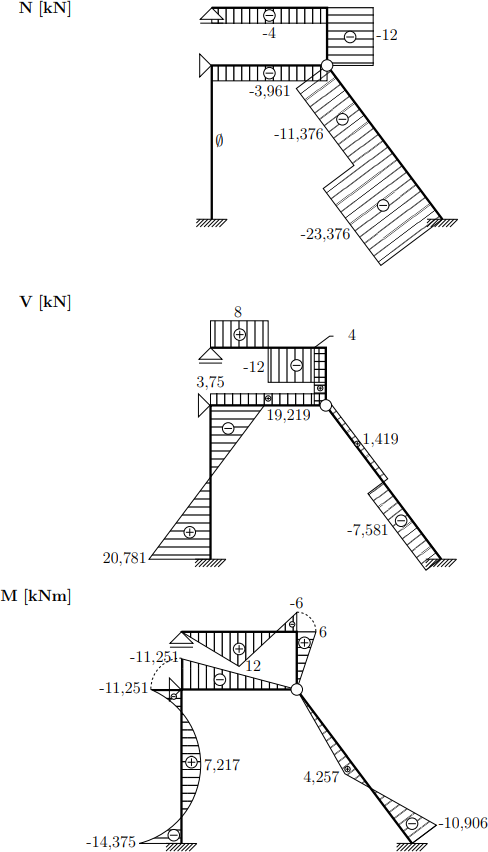
\includegraphics{assets/figures/framesss/example_internal_forces.png}
    \caption[Vnitřní síly na konstrukci]{Vnitřní síly na konstrukci, převzato z \cite[Příklad 5.2]{sbirka_prikladu}}
    \label{fig:framesss_example_internal_forces}
\end{figure}

\begin{table}[H]
    \setlength{\tabcolsep}{10pt}
    \renewcommand{\arraystretch}{1.2}
    \rowcolors{2}{ctulightblue!20}{white}
    \begin{tabular}{ccrrr}
        \rowcolor{ctulightblue} \bfseries veličina & \bfseries rozměr & \bfseries LC1 & \bfseries CO1 & \bfseries Sbírka \\ 
            $R_{1,\gls{x}}$ & $\SI{}{\kilo\newton}$ & -20.781 & -20.781 & -20.781 \\
            $R_{1,\gls{z}}$ & $\SI{}{\kilo\newton}$ &   0.000 &   0.000 &   0.000 \\
            \rowcolor{yellow!15}$M_{1,\gls{y}}$ & $\SI{}{\kilo\newton\metre}$ & -14.375 & -14.375 &  14.375 \\
            $R_{2,\gls{x}}$ & $\SI{}{\kilo\newton}$ & -15.258 & -15.258 & -15.258 \\
            \rowcolor{yellow!15}$R_{2,\gls{z}}$ & $\SI{}{\kilo\newton}$ &   3.750 &   3.750 &   -3.750 \\
            $R_{4,\gls{x}}$ & $\SI{}{\kilo\newton}$ &  -7.961 &  -7.961 &  -7.961 \\
            \rowcolor{yellow!15}$R_{4,\gls{z}}$ & $\SI{}{\kilo\newton}$ &  23.250 &  23.250 &  -23.249 \\
            \rowcolor{yellow!15}$M_{4,\gls{y}}$ & $\SI{}{\kilo\newton}$ &  10.905 &  10.905 &  -10.906 \\
            \rowcolor{yellow!15}$R_{6,\gls{z}}$ & $\SI{}{\kilo\newton}$ &   8.000 &   8.000 &  -8.000 \\
            $\gls{phi_i}[2]$ & $\SI{}{\radian}\cdot 10^{-5}$ & -6.942 & -6.942 & 6.942 \\
            \rowcolor{red!8}$\gls{u_i}[3]$ & $\SI{}{\metre}\cdot 10^{-5}$ & -9.902 & -9.902 & -9.903 \\
            \rowcolor{yellow!15}$\gls{w_i}[3]$ & $\SI{}{\metre}\cdot 10^{-4}$ & -9.168 & -9.168 & 9.168 \\
            $\gls{axial_force}_{1,2}$ & $\SI{}{\kilo\newton}$ & 0.000 & 0.000 & 0.000 \\
            %
            $\gls{axial_force}_{2,3}$ & $\SI{}{\kilo\newton}$ & -3.961 & -3.961 & -3.961 \\
            %
            $\min(\gls{axial_force}_{3,4})$ & $\SI{}{\kilo\newton}$ & -23.376 & -23.376 & -23.376 \\
            $\max(\gls{axial_force}_{3,4})$ & $\SI{}{\kilo\newton}$ & -11.376 & -11.376 & -11.376 \\
            %
            $\gls{axial_force}_{3,5}$ & $\SI{}{\kilo\newton}$ & -12.000 & -12.000 & -12.000 \\
            %
            $\gls{axial_force}_{6,5}$ & $\SI{}{\kilo\newton}$ & -4.000 & -4.000 & -4.000 \\
            %%%%%%%%%%%%%%%%%%%%%%%%%%%%%%%%%%%%%%%%%%%%%%%%%%%%%%%%%%%%%%%%%%%%%%%%%%%%%%%%%%%%%%%%%%
            $\min(\gls{shear_force}_{1,2})$ & $\SI{}{\kilo\newton}$ & -19.219 & -19.219 & -19.219 \\
            $\max(\gls{shear_force}_{1,2})$ & $\SI{}{\kilo\newton}$ & 20.781 & 20.781 & 20.781 \\
            %
            $\gls{shear_force}_{2,3}$ & $\SI{}{\kilo\newton}$ & 3.750 & 3.750 & 3.750 \\
            %
            $\min(\gls{shear_force}_{3,4})$ & $\SI{}{\kilo\newton}$ & -7.581 & -7.581 & -7.581 \\
            $\max(\gls{shear_force}_{3,4})$ & $\SI{}{\kilo\newton}$ & 1.419 & 1.419 & 1.419 \\
            %
            $\gls{shear_force}_{3,5}$ & $\SI{}{\kilo\newton}$ & 4.000 & 4.000 & 4.000 \\
            %
            $\min(\gls{shear_force}_{6,5})$ & $\SI{}{\kilo\newton}$ & -12.000 & -12.000 & -12.000 \\
            $\max(\gls{shear_force}_{6,5})$ & $\SI{}{\kilo\newton}$ & 8.000 & 8.000 & 8.000 \\
            %%%%%%%%%%%%%%%%%%%%%%%%%%%%%%%%%%%%%%%%%%%%%%%%%%%%%%%%%%%%%%%%%%%%%%%%%%%%%%%%%%%%%%%%%%
            $\min(\gls{bending_moment}_{1,2})$ & $\SI{}{\kilo\newton\meter}$ & -14.375 & -14.375 & -14.375 \\
            \rowcolor{red!8}$\max(\gls{bending_moment}_{1,2})$ & $\SI{}{\kilo\newton\meter}$ & 7.218 & 7.218 & 7.217 \\
            %
            $\min(\gls{bending_moment}_{2,3})$ & $\SI{}{\kilo\newton\meter}$ & -11.251 & -11.251 & -11.251 \\
            $\max(\gls{bending_moment}_{2,3})$ & $\SI{}{\kilo\newton\meter}$ & 0.000 & 0.000 & 0.000 \\
            %
            \rowcolor{red!8}$\min(\gls{bending_moment}_{3,4})$ & $\SI{}{\kilo\newton\meter}$ & -10.905 & -10.905 & -10.906 \\
            $\max(\gls{bending_moment}_{3,4})$ & $\SI{}{\kilo\newton\meter}$ & 4.257 & 4.257 & 4.257 \\
            %
            $\min(\gls{bending_moment}_{3,5})$ & $\SI{}{\kilo\newton\meter}$ & 0.000 & 0.000 & 0.000 \\
            $\max(\gls{bending_moment}_{3,5})$ & $\SI{}{\kilo\newton\meter}$ & 6.000 & 6.000 & 6.000 \\
            %
            $\min(\gls{bending_moment}_{6,5})$ & $\SI{}{\kilo\newton\meter}$ & -6.000 & -6.000 & -6.000 \\
            $\max(\gls{bending_moment}_{6,5})$ & $\SI{}{\kilo\newton\meter}$ & 12.000 & 12.000 & 12.000 
    \end{tabular}
    \caption{Porovnání výsledků}
    \label{tab:example_values}
\end{table}

V \autoref{tab:example_values} jsou uvedeny hodnoty vypočítané knihovnou \texttt{framesss} a srovnány s referenčními hodnotami ze \textit{Sbírky příkladů stavební mechaniky} \cite{sbirka_prikladu}. Testování probíhalo ve dvou různých scénářích: zatěžovací stav (LC1) a kombinace zatěžovacích stavů (CO1). LC1 představuje stav, kde je veškeré zatížení aplikováno najednou. CO1 je kombinace jednotlivých zatěžovacích stavů, kde každé zatížení bylo odděleně definováno a hodnota zatížení byla vydělena předem definovaným součinitel. Následně byly tyto zatěžovací stavy zkombinovány do kombinace zatěžovacích stavů s těmito součiniteli.

Porovnání výsledků ukazuje, že hodnoty vypočítané knihovnou \texttt{framesss} jsou téměř stejné jako referenční hodnoty, přičemž rozdíly (vyznačené \colorbox{red!8}{červenou barvou}) se nacházejí v rámci zaokrouhlovací chyby.

Hodnoty posunutí a reakcí ve směru osy \gls{Z} a hodnoty pootočení a momentů okolo osy \gls{Y} vykazují opačné znaménko (vyznačeno \colorbox{yellow!15}{žlutou barvou}) ve srovnání s referenčními hodnotami, což je způsobeno rozdílným natočením globálního souřadného systému, viz obr. \ref{fig:example_coordinate_systems}. Systém ze sbírky je vlevo, uvažovaný systém při zadávání konstrukce v této práci vpravo. Při stanovení kladného směru pootočení platí pravidlo pravé ruky.

\begin{figure}[H]
    \begin{tikzpicture}[>={Stealth[inset=0pt,length=8pt,angle'=28,round]}]
    \draw[->] (0, 0) -- ++(2,0) node[above right=0 and -1] {$+\gls{X}$, $+\gls{u_i}$, $+R_{\gls{x},i}$};
    \draw[->] (0, 0) -- ++(0,-2) node[right] {$+\gls{Z}$, $+\gls{w_i}$, $+R_{\gls{z},i}$};
    \draw[->,domain=180:450] plot ({cos(\x)}, {sin(\x)}) node[above] {$+\gls{phi_i}$, $+R_{M,\gls{y},i}$};

    \draw[->] (6, 0) -- ++(2,0) node[above right=0 and -1] {$+\gls{X}$, $+\gls{u_i}$, $+R_{\gls{x},i}$};
    \draw[->] (6, 0) -- ++(0,2) node[right] {$+\gls{Z}$, $+\gls{w_i}$, $+R_{\gls{z},i}$};
    \draw[->,domain=180:-90] plot ({6+cos(\x)}, {sin(\x)}) node[below] {$+\gls{phi_i}$, $+R_{M,\gls{y},i}$};
\end{tikzpicture}
    \caption{Porovnání souřadných systémů}
    \label{fig:example_coordinate_systems}
\end{figure}

